\documentclass{beamer}
\usepackage[utf8]{inputenc}
\usepackage[T1]{fontenc}
\usepackage{listings}
\usepackage{graphicx}
\usepackage{placeins}
\usetheme{Madrid}

\author{Renê Cardozo - 9797315 \\ 
        Verônica Stocco - 6828626 \\
        rene.cardozo@usp.br \\
        veronica.stocco@usp.br}

\title{EP1}
\institute{Instituto de Matemática e Estatística \\
Universidade de São Paulo}

\date{}

\begin{document}
\frame{\titlepage}

\begin{frame}

\frametitle{BCCSH}

O executável bccsh é composto de dois módulos: parser e bccsh. Além disso é utilizada a biblioteca readline, a qual tem
seu caminho encontrado pela ferramenta pkgconfig.

\end{frame}

\begin{frame}
\frametitle{Parser}

\begin{itemize}
\item O parser é responsável por receber a linha de caracteres retornada pela função readline da biblioteca readline e separar cada palavra em um vetor de argumentos, os quais serão reconhecidos pelo bccsh posteriormente e determinarão qual comando deverá ser executado.  

\item Este parser foi adotado pensando em possibilitar a execução de qualquer binário pelo shell, bem como unificar o processo de execução de comandos internos e outros programas do sistema.  


\item Há uma limitação de 10 strings para cada linha lida pelo parser.

\end{itemize}
\end{frame}

\begin{frame}

\begin{itemize}
\frametitle{Shell}
\item O shell propriamente dito é implementado no arquivo bccsh.c, o qual realiza a leitura de inputs pelo usuário utilizando
a função readline, sendo lida uma linha por vez. 

\item Após o armazenamento da linha em um buffer, caso a linha não seja
vazia, esta será armazenada no histórico através da função add\_history da biblioteca readline, podendo ser acessada,
por padrão, utilizando as setas do teclado.

\end{itemize}
\end{frame}

\begin{frame}
\frametitle{Comandos}

Uma vez salvo no histórico, a linha será utilizada pelo parser para criar um vetor com as palavras digitadas. As quais
utilizarão a função cmd para determinar qual comando será executado. Podendo este ser:

\begin{itemize}
    \item mkdir <diretório>
    \item kill -<sinal> <PID>
    \item ln -s <arquivo> <link>
    \item Qualquer binário do sistema iniciado por "/" ou ".", com no máximo 9 argumentos.
\end{itemize}
\end{frame}

\begin{frame}
\frametitle{Escalonador de Processos}
O simulador de escalonamento de processos é definido no arquivo ep1.c, no qual estão definidas as rotinas de
    escalonamento com os algoritmos First-Come, First-Served (FCFS) e Shortest Remaining Time Next (SRTN).

\begin{block}{Round-Robin}
O algoritmo Round-Robin está apenas no esboço de uma tentativa de implementação, contudo não foi possível testá-lo como
os outros e sua execução não está correta.
\end{block}

Neste arquivo é utilizada a função read\_file para ler os arquivos da pasta entrada, na qual são armazenados os arquivos
criados pelo gerador de processos, os quais são organizados em um array de structs onde é armazenado o nome, t0, dt e
    deadline de cada processo.
\end{frame}

\begin{frame}
\frametitle{Algoritmos de Escalonamento}
A partir do primeiro parâmetro fornecido para o executável ./ep1 temos a escolha do algoritmo que será utilizado na
    simulação, sendo 1 para FCFS e 2 para SRTN.

A implementação dos algoritmos foi feita da seguinte forma:
\begin{itemize}
    \item FCFS: Executa as threads diretamente do array de processos montado na leitura, uma vez que supõe-se que os processos estejam ordenados por ordem de chegada.
    \item SRTN: Reordena o array de processos com base na soma dos atributos t0 e dt, assim, priorizam-se os processos
        com menor dt que chegam antes.
    \item RR: Cria as threads e envia um sinal para que a primeira possa executar. A thread i executa por um quantum, e envia um signal 
    para que a thread (i + 1) \% process\_count possa executar. 

\end{itemize}

Os algoritmos armazenam a saída no arquivo especificado pelo terceiro parâmetro do executável ./ep1, no qual é escrito o
nome do processo o tempo atual do simulador e o tempo do simulador menos o tempo inicial do processo.

\end{frame}

\begin{frame}
\frametitle{Gerador de Processos}
A criação de processos para uso pelo simulador é feito pelo arquivo gerador.c dentro da pasta gerador\_de\_processos.
    Este programa é executado da forma "./gerador <número-de-processos> [semente]", sendo a semente opcional e por
    padrão igual a 0.
\begin{itemize}
    \item t0 inicia-se com 1 e é incrementado em um inteiro aleatório entre 0 e 3.
    \item dt é gerado como um inteiro aleatório entre 2 e 5.
    \item a deadline do processo é gerada por t0 + dt + x, sendo x um número inteiro aleatório entre 0 e 15.
\end{itemize}
\end{frame}

\begin{frame}
\frametitle{Testes}
Os testes foram realizados a partir da geração de três arquivos de processos, com 5, 50 e 500 processos.

A execução de cada teste foi realizada para os dois algoritmos implementados e executadas trinta vezes para cada arquivo
de 5, 50 e 500 processos.

A execução usou como base:
\begin{itemize}
    \item ./bccsh
    \item ./ep1 <1 ou 2> entrada/<arquivo-de-entrada> saida/<arquivo-de-saida> d
\end{itemize}

\end{frame}

\begin{frame}
\frametitle{Máquinas Utilizadas}

Foram utilizadas duas máquinas diferentes, uma com 12 e outra com 8 CPUs, as quais estão descritas nos slides a seguir, que registram as saídas do comando lscpu para cada uma das máquinas.


\begin{block}{Limitações}
A máquina 1, com 12 núcleos, sofreu aparente limitação pela utilização do Windows Subsystem for Linux, uma vez que
    apenas uma CPU parece ter sido utilizada, o que pode ser observado pela saída "0" no modo verboso do simulador.
\end{block}
\end{frame}

\begin{frame}
\frametitle{Máquina 1}

\begin{columns}
\begin{column}{0.7\textwidth}
\scriptsize{Architecture:        x86\_64\\
CPU op-mode(s):      32-bit, 64-bit\\
Byte Order:          Little Endian\\
Address sizes:       36 bits physical, 48 bits virtual\\
CPU(s):              12\\
On-line CPU(s) list: 0-11\\
Thread(s) per core:  2\\
Core(s) per socket:  6\\
Socket(s):           1\\
Vendor ID:           GenuineIntel\\
CPU family:          6\\
Model:               158\\
Model name:          Intel(R) Core(TM) i7-9750H CPU @ 2.60GHz\\
Stepping:            10\\
CPU MHz:             2601.000\\
CPU max MHz:         2601.0000\\
BogoMIPS:            5202.00\\
Virtualization:      VT-x\\
Hypervisor vendor:   Windows Subsystem for Linux\\
Virtualization type: container\\}
\end{column}
\begin{column}{0.3\textwidth}
\scriptsize{Flags:               fpu vme de pse tsc msr pae mce cx8 apic sep mtrr pge mca cmov pat pse36 clflush dts acpi mmx fxsr sse sse2 ss ht tm pbe syscall nx pdpe1gb rdtscp lm pni pclmulqdq dtes64 monitor ds\_cpl vmx est tm2 ssse3 fma cx16 xtpr pdcm pcid sse4\_1 sse4\_2 x2apic movbe popcnt tsc\_deadline\_timer aes xsave osxsave avx f16c rdrand lahf\_lm abm 3dnowprefetch fsgsbase tsc\_adjust bmi1 avx2 smep bmi2 erms invpcid mpx rdseed adx smap clflushopt intel\_pt ibrs ibpb stibp ssbd}
\end{column}
\end{columns}
\end{frame}

\begin{frame}
\frametitle{Máquina 2}

\begin{columns}
\begin{column}{0.7\textwidth}
\scriptsize{
Architecture:          x86\_64 \\
CPU op-mode(s):        32-bit, 64-bit\\
Byte Order:            Little Endian\\
CPU(s):                8\\
On-line CPU(s) list:   0-7\\
Thread(s) per core:    2\\
Core(s) per socket:    4\\
Socket(s):             1\\
NUMA node(s):          1\\
Vendor ID:             GenuineIntel\\
CPU family:            6\\
Model:                 42\\
Model name:            Intel(R) Core(TM) i7-2700K CPU @ 3.50GHz\\
Stepping:              7\\
CPU MHz:               4393.984\\
CPU max MHz:           4600,0000\\
CPU min MHz:           1600,0000\\
BogoMIPS:              6984.19\\
Virtualization:        VT-x\\
L1d cache:             32K\\
L1i cache:             32K\\
L2 cache:              256K\\
L3 cache:              8192K\\
NUMA node0 CPU(s):     0-7\\}
\end{column}
\begin{column}{0.3\textwidth}
\scriptsize{Flags:                 fpu vme de pse tsc msr pae mce cx8 apic sep mtrr pge mca cmov pat pse36 clflush dts acpi mmx fxsr sse sse2 ss ht tm pbe syscall nx rdtscp lm constant\_tsc arch\_perfmon pebs bts rep\_good nopl xtopology nonstop\_tsc cpuid aperfmperf pni pclmulqdq dtes64 monitor ds\_cpl vmx est tm2 ssse3 cx16 xtpr pdcm pcid sse4\_1 sse4\_2 popcnt tsc\_deadline\_timer aes xsave avx lahf\_lm epb pti ssbd ibrs ibpb stibp tpr\_shadow vnmi flexpriority ept vpid xsaveopt dtherm ida arat pln pts md\_clear flush\_l1d}
\end{column}
\end{columns}
\end{frame}

\begin{frame}
\frametitle{Gráficos de Deadline}


\begin{figure}[!htb]
\minipage{0.32\textwidth}
  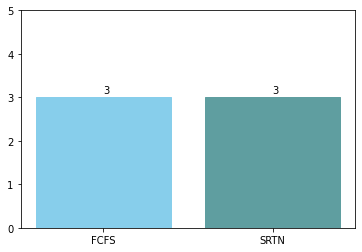
\includegraphics[width=\linewidth]{imgs/deadline5-1}
  \caption{M1, 5 threads}\label{fig:awesome_image1}
\endminipage\hfill
\minipage{0.32\textwidth}
  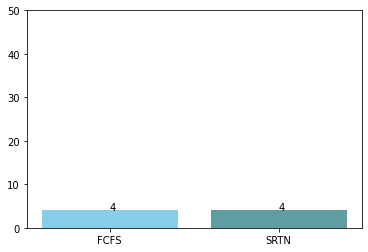
\includegraphics[width=\linewidth]{imgs/deadline50-1}
  \caption{M1, 50 threads}\label{fig:awesome_image2}
\endminipage\hfill
\minipage{0.32\textwidth}%
  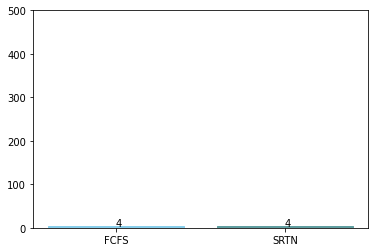
\includegraphics[width=\linewidth]{imgs/deadline500-1}
  \caption{M1, 500 threads}\label{fig:awesome_image3}
\endminipage
\end{figure}





\begin{figure}[!htb]
\minipage{0.32\textwidth}
  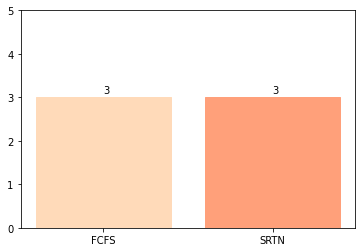
\includegraphics[width=\linewidth]{imgs/deadline5-2}
  \caption{M2, 5 threads}\label{fig:awesome_image1}
\endminipage\hfill
\minipage{0.32\textwidth}
  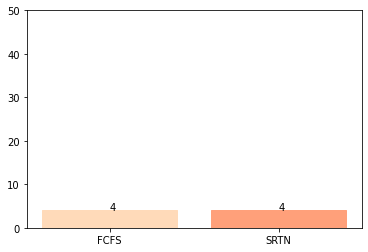
\includegraphics[width=\linewidth]{imgs/deadline50-2}
  \caption{M2, 50 threads}\label{fig:awesome_image2}
\endminipage\hfill
\minipage{0.32\textwidth}%
  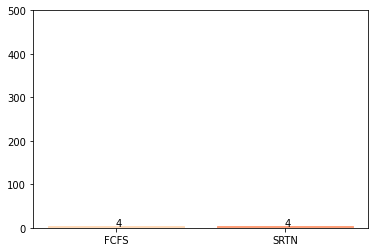
\includegraphics[width=\linewidth]{imgs/deadline500-2}
  \caption{M2, 500 threads}\label{fig:awesome_image3}
\endminipage
\end{figure}


\end{frame}

\begin{frame}
\frametitle{Gráficos de Mudanças de Contexto: Análise}

Os resultados \textbf{não} foram os esperados.

\begin{itemize}
\item Era de se esperar que o SRTN cumprisse mais deadlines que o FCFS. Além disso não acontecer, ambos escalonadores apresentaram \textit{exatamente} o mesmo desempenho em \textbf{todas} as execuções do código. 

\item Após analisar os resultados e revisitar o código, identificamos o motivo do erro. Ao invés de implementar o SRTN (que deveria suspender um processo quando um mais curto chegasse), implementamos o Shortest Remaining Time First (ordenamos o vetor de processos com base no t0 + dt, mas não houve qualquer comunicação entre as threads para que o processo mais curto disponível interrompesse a execução do processo atual). Infelizmente, quando nos demos conta disso, não havia mais tempo para corrigir a implementação.
\end{itemize}

\end{frame}


\begin{frame}
\frametitle{Gráficos de Mudanças de Contexto: Análise}

\begin{itemize}
\item \textbf{(Falta de) diferença entre as máquinas:} era esperado que o desempenho em ambas fosse o mesmo. Não havia threads correndo em paralelo, já que nossa implementação simulava apenas 1 CPU.

\item \textbf{(Falta de) diferença entre as execuções:} \textit{não} era esperado que todas as execuções levassem a exatamente os mesmos resultados. Deveriam ter havido ocasiões em que mais de uma thread poderia ter acesso ao mutex, o que levaria a resultados diferentes. Entretanto, os processos sempre foram executados na ordem [0, 1, 2, ..., n]. Como todas as 30 execuções levaram ao mesmo resultado, não fazia sentido incluir a média e intervalo de confiança nos gráficos.

\item Acreditamos que isso se deve ao fato de cada pthread\_join ter sido dentro do loop de criação de cada thread. Ou seja: cada thread foi concluída logo após sua criação. Não haviam threads existentes simultaneamente, o que impediu que duas ou mais threads pudessem entrar em condição de corrida, que seria o motivo de ter resultados diferentes em diferentes execuções.
\end{itemize}

\end{frame}

\begin{frame}
\frametitle{Gráficos de Mudanças de Contexto: Análise}
\begin{itemize}
\item A baixíssima taxa de cumprimento de deadlines também não era esperada. Isso foi um problema com os arquivos de entrada que utilizamos, e não com o algoritmo. Todos os deadlines que geramos automaticamente eram muito curtos e muito próximos, e não poderiam ser cumpridos em tempo por uma máquina com uma única CPU.

\item Se tivéssemos gerado prazos maiores para os processos, ou simulados mais CPUs, mais deadlines teriam sido cumpridos. 
\end{itemize}
\end{frame}


\begin{frame}
\frametitle{Gráficos de Mudanças de Contexto}


\begin{figure}[!htb]
\minipage{0.32\textwidth}
  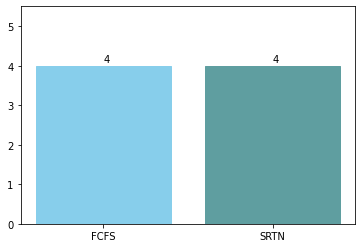
\includegraphics[width=\linewidth]{imgs/contex5-1}
  \caption{M1, 5 threads}\label{fig:awesome_image1}
\endminipage\hfill
\minipage{0.32\textwidth}
  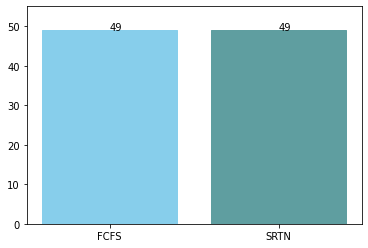
\includegraphics[width=\linewidth]{imgs/contex50-1}
  \caption{M1, 50 threads}\label{fig:awesome_image2}
\endminipage\hfill
\minipage{0.32\textwidth}%
  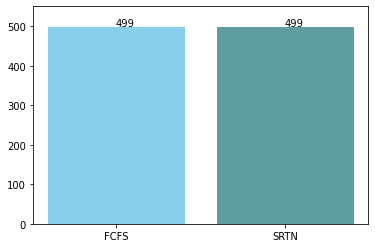
\includegraphics[width=\linewidth]{imgs/contex500-1}
  \caption{M1, 500 threads}\label{fig:awesome_image3}
\endminipage
\end{figure}



\begin{figure}[!htb]
\minipage{0.32\textwidth}
  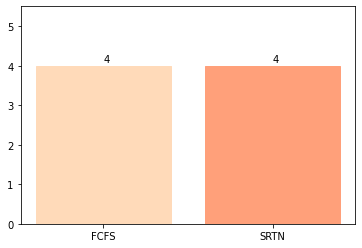
\includegraphics[width=\linewidth]{imgs/contex5-2}
  \caption{M2, 5 threads}\label{fig:awesome_image1}
\endminipage\hfill
\minipage{0.32\textwidth}
  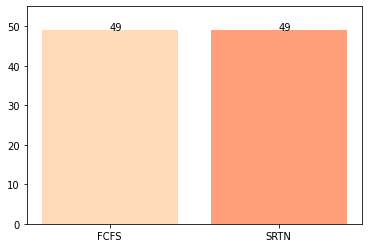
\includegraphics[width=\linewidth]{imgs/contex50-2}
  \caption{M2, 50 threads}\label{fig:awesome_image2}
\endminipage\hfill
\minipage{0.32\textwidth}%
  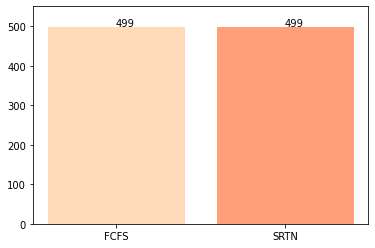
\includegraphics[width=\linewidth]{imgs/contex500-2}
  \caption{M2, 500 threads}\label{fig:awesome_image3}
\endminipage
\end{figure}

\end{frame}




\begin{frame}
\frametitle{Gráficos de Mudanças de Contexto: Análise}

Mais uma vez, os resultados \textbf{não} foram os esperados.

\begin{itemize}
\item Se houvéssemos implementado o SRTN da forma correta, ele apresentaria mais mudanças de contexto que o FCFS. Entretanto, considerando que (infeliz e erroneamente) implementamos o Shortest Remaining Time Next, faz sentido que o número de mudanças de contexto seja o mesmo do escalonador FCFS.

\item Como explicado no gráfico anterior, suspeitamos que utilizamos o pthread\_join de forma errada, o que levou à ausência de qualquer condição de corrida entre threads. Tendo isso em vista, faz sentido que todos os resultados mais uma vez tenham sido idênticos.

\end{itemize}

\end{frame}

\end{document}

